\RequirePackage[l2tabu,orthodox]{nag}

% TODO: decide if one-sided/two-sided
%\documentclass[headsepline,footsepline,footinclude=false,fontsize=11pt,paper=a4,listof=totoc,bibliography=totoc,BCOR=12mm,DIV=12]{scrbook} % two-sided
\documentclass[headsepline,footsepline,footinclude=false,oneside,fontsize=11pt,paper=a4,listof=totoc,bibliography=totoc]{scrbook} % one-sided

\PassOptionsToPackage{table,svgnames,dvipsnames}{xcolor}

\usepackage[utf8]{inputenc}
\usepackage[T1]{fontenc}
\usepackage[sc]{mathpazo}
\usepackage[american]{babel}
\usepackage[autostyle]{csquotes}
\usepackage[%
  backend=biber,
  url=false,
  style=alphabetic,
  maxnames=4,
  minnames=3,
  maxbibnames=99,
  firstinits,
  uniquename=init]{biblatex} % TODO: adapt bibliography style
\usepackage{graphicx}
\usepackage{scrhack} % necessary for listings package
\usepackage{listings}
\usepackage{lstautogobble}
\usepackage{tikz}
\usepackage{pgfplots}
\usepackage{pgfplotstable}
\usepackage{booktabs}
\usepackage[final]{microtype}
\usepackage{caption}
\usepackage[hidelinks]{hyperref} % hidelinks removes colored boxes around references and links
\addto\extrasenglish{%
  \def\chapterautorefname{Chapter}%
  \def\sectionautorefname{Section}%
}

%\usepackage{cleveref}
\usepackage[toc,nonumberlist,acronym]{glossaries} % TODO: remove if glossary not needed

\usepackage{color}
\usepackage[section]{placeins}
\usepackage{float}
\usepackage{xcolor}

\usepackage{pgf-umlsd}
\usetikzlibrary{arrows,shadows,snakes,backgrounds}

\usepackage{verbatim}
\usepackage{pbox}

\bibliography{bibliography/literature}

\setkomafont{disposition}{\normalfont\bfseries} % use serif font for headings
\linespread{1.05} % adjust line spread for mathpazo font

% Settings for glossaries TODO: remove the following block if glossary not needed
\renewcommand{\glsnamefont}[1]{\normalfont\bfseries #1} % use serif font for glossary entry titles
\makeglossaries{}

% Settings for pgfplots
\pgfplotsset{compat=1.9} % TODO: adjust to your installed version
\pgfplotsset{
  % For available color names, see http://www.latextemplates.com/svgnames-colors
  cycle list={CornflowerBlue\\Dandelion\\ForestGreen\\BrickRed\\},
}

\definecolor{pblue}{rgb}{0.13,0.13,1}
\definecolor{pgreen}{rgb}{0,0.5,0}
\definecolor{pred}{rgb}{0.9,0,0}
\definecolor{pgrey}{rgb}{0.46,0.45,0.48}

\colorlet{punct}{red!60!black}
\definecolor{background}{HTML}{EEEEEE}
\definecolor{delim}{RGB}{20,105,176}
\colorlet{numb}{magenta!60!black}


% \lstdefinestyle{customJava}{
% belowcaptionskip=1\baselineskip,
% breaklines=true,
% frame=L,
% xleftmargin=\parindent,
% language=Java,
% showstringspaces=false,
% showspaces=false,
% backgroundcolor=\color{background},
% breakatwhitespace=true,
% basicstyle=\footnotesize\ttfamily,
% commentstyle=\color{pgreen},
% keywordstyle=\color{pblue},
% stringstyle=\color{pred},
% moredelim=[il][\textcolor{pgrey}]{\$},
% moredelim=[is][\textcolor{pgrey}]{\%\%}{\%\%}
% }

\lstdefinestyle{customJava}{
basicstyle=\normalfont\ttfamily,
belowcaptionskip=1\baselineskip,
numbers=left,
numberstyle=\scriptsize,
stepnumber=1,
numbersep=8pt,
breaklines=true,
frame=lines,
xleftmargin=\parindent,
language=Java,
showstringspaces=false,
showspaces=false,
backgroundcolor=\color{background},
breakatwhitespace=true,
commentstyle=\color{pgreen},
keywordstyle=\color{pblue},
stringstyle=\color{pred},
moredelim=[il][\textcolor{pgrey}]{\$},
moredelim=[is][\textcolor{pgrey}]{\%\%}{\%\%}
}

\lstdefinelanguage{json}{
basicstyle=\normalfont\ttfamily,
numbers=left,
numberstyle=\scriptsize,
stepnumber=1,
numbersep=8pt,
showstringspaces=false,
breaklines=true,
frame=lines,
backgroundcolor=\color{background},
literate=
*{0}{{{\color{numb}0}}}{1}
{1}{{{\color{numb}1}}}{1}
{2}{{{\color{numb}2}}}{1}
{3}{{{\color{numb}3}}}{1}
{4}{{{\color{numb}4}}}{1}
{5}{{{\color{numb}5}}}{1}
{6}{{{\color{numb}6}}}{1}
{7}{{{\color{numb}7}}}{1}
{8}{{{\color{numb}8}}}{1}
{9}{{{\color{numb}9}}}{1}
{:}{{{\color{punct}{:}}}}{1}
{,}{{{\color{punct}{,}}}}{1}
{\{}{{{\color{delim}{\{}}}}{1}
{\}}{{{\color{delim}{\}}}}}{1}
{[}{{{\color{delim}{[}}}}{1}
{]}{{{\color{delim}{]}}}}{1},
}

% Settings for lstlistings
\lstset{%
  basicstyle=\ttfamily,
  columns=fullflexible,
  autogobble,
  style=customJava
}

\FloatBarrier

% Basic information for cover & title page
\newcommand*{\getUniversity}{Technische Universität München}
\newcommand*{\getFaculty}{Fakultät für Informatik}
\newcommand*{\getTitle}{Refactoring an Orchestration Microservice for Simplicity of Control Flow Definition and Customizability.}
\newcommand*{\getTitleGer}{Refactoring einer Orchestrierungsmicroservice zur Vereinfachung der Kontrollfluss Definition und Anpassbarkeit.}
\newcommand*{\getAuthor}{Rajendra Kharbuja}
\newcommand*{\getDoctype}{Master’s Thesis in Informatics}
\newcommand*{\getSupervisor}{Prof. Dr. Florian Matthes}
\newcommand*{\getAdvisor}{Dr. Holger Wittges}
\newcommand*{\getSubmissionDate}{}
\newcommand*{\getSubmissionLocation}{Munich}

% TODO: add custom commands etc.


\makeglossaries
\newglossaryentry{computer}
{
  name=computer,
  description={is a machine that\ldots}
}
 
\newacronym{DDE}{DDE}{Dart Dart Everywhere}
\newacronym{uuid}{UUID}{Universally Unique Identifier}
\newacronym{uri}{URI}{Uniform Resource Identifier}
\newacronym{VM}{VM}{Virtual Machine}
\newacronym{MQS}{MQS}{Message Queuing System}
\newacronym{MBS}{MBS}{Message Broker System}
\newacronym{JSON}{JSON}{JavaScript Object Notation}
\newacronym{RTT}{RTT}{Round Trip Time}


\begin{document}

\begin{titlepage}
  % HACK for two-sided documents: ignore binding correction for cover page.
  % Adapted from Markus Kohm's KOMA-Script titlepage=firstiscover handling.
  % See http://mirrors.ctan.org/macros/latex/contrib/koma-script/scrkernel-title.dtx,
  % \maketitle macro.
  \oddsidemargin=\evensidemargin\relax
  \textwidth=\dimexpr\paperwidth-2\evensidemargin-2in\relax
  \hsize=\textwidth\relax

  \centering

  \vspace{40mm}
  
\includegraphics[width=40mm]{logos/tum}

  \vspace{5mm}
  {\huge\MakeUppercase{\getFaculty{}}}\\

  \vspace{5mm}
  {\large\MakeUppercase{\getUniversity{}}}\\

  \vspace{20mm}
  {\Large \getDoctype{}}

  \vspace{15mm}
  {\large \getTitle{}} %{\huge\bfseries \getTitle{}}

  \vspace{15mm}
  {\LARGE \getAuthor{}}

  \vspace{20mm}
  
\includegraphics[width=20mm]{logos/faculty}
\end{titlepage}


\frontmatter{}

\begin{titlepage}
  \centering

  \vspace{40mm}
  
\includegraphics[width=40mm]{logos/tum}

  \vspace{5mm}
  {\huge\MakeUppercase{\getFaculty{}}}\\

  \vspace{5mm}
  {\large\MakeUppercase{\getUniversity{}}}\\

  \vspace{18mm}
  {\Large \getDoctype{}}

  \vspace{13mm}
  {\large \getTitle{}} %{\huge\bfseries \getTitle{}}

  \vspace{8mm}
  {\large \getTitleGer{}} %{\huge\bfseries \getTitleGer{}}

  \vspace{15mm}
  \begin{tabular}{l l}
    Author: & \getAuthor{} \\
    Supervisor: & \getSupervisor{} \\
    Advisor: & \getAdvisor{} \\
    Submission Date: & \getSubmissionDate{} \\
  \end{tabular}

  \vspace{12mm} %20mm
  
\includegraphics[width=20mm]{logos/faculty}
\end{titlepage}

\thispagestyle{empty}
\vspace*{0.8\textheight}
\noindent
 I confirm that this \MakeLowercase{\getDoctype{}} is my own work and I have documented all sources and material used.

\vspace{15mm}
\noindent
\getSubmissionLocation{}, \getSubmissionDate{} \hspace{5cm} \getAuthor{}

\cleardoublepage{}

\addcontentsline{toc}{chapter}{Acknowledgments}
\thispagestyle{empty}

\vspace*{2cm}

\begin{center}
{\usekomafont{section} Acknowledgments}
\end{center}

\vspace{1cm}

\cleardoublepage{}

\chapter{\abstractname}

\microtypesetup{protrusion=false}
\tableofcontents{}
\microtypesetup{protrusion=true}

\mainmatter{}

\chapter{Introduction}\label{chapter:introduction}

\section{Motivation}\label{section:introduction/motivation}
%software architecture and its objectives, relating to responding to the change
Software Architecture definition is an inevitable and crucial step for software development process. By defining an architecture, we define elements, their behavior, their structural composition to construct a system as a whole and various interfaces to characterize communication required between the elements. \cite{microsoft1501} The objective of building an architecture is not only to provide the desired functionalities but also to calibrate the quality of the software across various non-functional attributes such as availability, usability, performance etc. Modifiability is one among the various other quality attributes controlled by an architecture. \cite{Wesley0301}


Software development process as well as development pattern play an equal role to define quality attributes. The quality attributes can be broadly classified as a)Structural and b)Process quality attributes. The structural quality attributes such as testability, modifiability, security etc are affected by the development pattern followed by developers. Adoption of a specific design pattern to solve a problem may be one example of a significant development approach. Similarly, the quality attributes are affected differently, based on the development methodology used. For example, an agile methodology will help to improve maintainability due to its approach of getting fast customer response.\cite{Chappell01}

%change as the most probable expectation and impact of change
Software change is unavoidable for many reasons. The changes are driven by difference between the software’s ability and expectations along time. Additionally, the focus on growing the software require it to undergo changes. Another reason can be to nullify the technical debt occurred along the development stages due to various compromising decisions made.\cite{elsevier0901}
A research carried out by Agile Manifesto, whose result is shown by figure\ref{fig:requirementmismatch} suggests that a surprisingly higher percentage of projects actually fail to meet the requirements of the user.
\begin{figure}[H]
\begin{center}
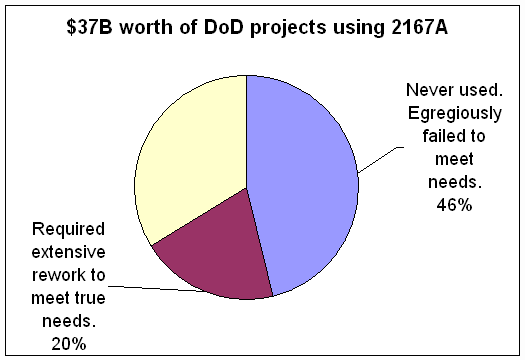
\includegraphics[width=0.8\textwidth]{figures/introduction-motivation}
\caption{Percentage of Projects with Requirement mismatch \cite{Miyachi01}}
\label{fig:requirementmismatch}
\end{center}
\end{figure}
However, responding to change is not free and impose significant impact on software architecture and development methodology. The purpose of architecture and development methodology should be to incorporate those changes and lower the technical debt as swiftly as possible.\cite{Northrop1501} Any variation to software architecture affects coupling and cohesion and thus impacting understandability as well as complexity of the software.\cite{elsevier0901}

The software development methodologies have come a long way undergoing a lot of modifications. Few of them to list would be waterfall model, spiral model, \acrshort{RAD} model and iterative model.\cite{CMS0801} Nevertheless, we have agile modeling, which works around some basic principles. Accepting change requirement at any stage of development and releasing software regularly are among the principles which supports to reduce the the cost of change.\cite{StellmanGreene1401}	

%evolution of the software architecture and development methodology %SOA and microservices
Accordingly, software architecture has changed in number of ways and in number of direction throughout the history of evolution. It has passed through monolithic, layered, distributed object, domain driven development, hexagonal, service oriented architecture etc. \cite{Sommerville0401} Nonetheless, we have microservices architecture with one of the major driving concepts being to improve cohesion and decrease coupling among components. This eventually, apart from accomplishing various other major goals, also upgrades the rate and efficiency of customizability.\cite{Newman1501}

%orchestration micro service is not an exception to that
Microservices are achieved by breaking down a system along business domains following Single Responsibility Principle. As the individual microservices achieved in such a way become the autonomous components, there is a need for a separate kind of component micro service in order to fulfill high-level business goals, which is Orchestration microservice. \cite{Newman1501} Regardless of following agile development methodology and microservice architecture, orchestration has been a painful and cumbersome area, considering the complexities being suffered when one has to make changes at any given point. There are a lot of technological and conceptual procedures around orchestration to make it less painful but at the same time there is no single agreement upon which one to follow.\cite{DanielPernici0601}


% later\chapter{Literature Review}\label{chapter:literature_review}
\section{Software Architecture}\label{section:software_architecture}


\begin{definition}[Software architecture \cite{bass_sa}]



%later\chapter{System Design}
\label{chapter:system_design}
%later\chapter{Results}
\label{chapter:results}

%later\chapter{Discussions}\label{chapter:discussions}
%later\chapter{Conclusion}\label{chapter:conclusion}
% What you learned
% What went well, bad, surprises, insights
% How you'd do it differently?
%later\chapter{Future Directions}\label{chapter:future_directions}
%later\chapter{Appendices}\label{chapter:appendices}

\section{TODO}
% How to setup and startup the system -> From GitHub Readme
% Some screenshots of the Registry showing connected nodes
% Tables of the benchamark-charts?


\appendix{}

\glsaddall{} % add all defined terms to glossary, even if not referenced in text
%\printglossaries{}
\printglossary[type=\acronymtype]

\microtypesetup{protrusion=false}
\listoffigures{}
%later\listoftables{}
\microtypesetup{protrusion=true}
\printbibliography{}

\end{document}
